\documentclass[12pt]{article}

\usepackage[ngerman]{babel}
\usepackage[babel,german=swiss]{csquotes} % Schweizer

\usepackage{amsmath}
\usepackage{graphicx}
\usepackage{array}
\usepackage{fancyhdr}
\usepackage{xcolor}
\usepackage{graphicx}
\usepackage{wrapfig}
\usepackage{tabularx}
\usepackage{float}
\usepackage{natbib}

\usepackage{fontspec,xltxtra,xunicode}
\defaultfontfeatures{Mapping=tex-text}
\setromanfont[Mapping=tex-text]{Calibri}
\setsansfont[Scale=MatchLowercase,Mapping=tex-text]{Gill Sans}
\setmonofont[Scale=MatchLowercase]{Andale Mono}
\linespread{1.2}

% PDF Einstellungen
\usepackage[draft=false, debug=false]{hyperref}
\hypersetup{
	pdfauthor={Michael Höhn, Stefan Hauenstein},
	pdftitle={Projektarbeit: Doppelt inverses Pendel},
	bookmarks,
	colorlinks,%
    citecolor=black,%
    filecolor=black,%
    linkcolor=black,%
    urlcolor=black
}

\usepackage[paper=a4paper]{geometry} 

% Heading Layout
\pagestyle{fancy}
\fancyhf{}
\fancyhead[L]{Projektarbeit: Doppelt inverses Pendel}
\fancyfoot[C]{\thepage}
\renewcommand{\headrulewidth}{0.1pt}
\renewcommand{\footrulewidth}{0.0pt}
\setcounter{secnumdepth}{4}
\setlength{\headheight}{15pt}

% Paragraph
\setlength\parindent{0pt} 
\setlength{\parskip}{0.75em}

% set graphics
\graphicspath{{./images/}}
\DeclareGraphicsExtensions{.png, .jpg}

% set equation numbering
\numberwithin{equation}{subsection}

% No dots in TOC
\makeatletter \renewcommand{\@dotsep}{10000} \makeatother

\title{\vspace{-1cm}\linespread{1}\begin{flushleft}\normalsize{Zürcher Hochschule für Angewandte Wissenschaften\\Studiengang Informatik\\}\end{flushleft}\vspace{2cm}\Large{Projektarbeit: Doppelt inverses Pendel}\\\vspace{2cm} 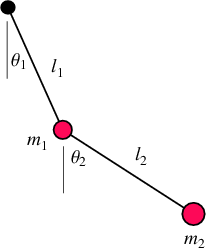
\includegraphics[scale=1]{title.png}\\\tiny{Bild: scienceworld.wolfram }}

\author{Michael Höhn\\\href{mailto:hoehnmic@students.zhaw.ch}{hoehnmic@students.zhaw.ch} \and Stefan Hauenstein\\\href{mailto:hauenste@students.zhaw.ch}{hauenste@students.zhaw.ch}}

\date{\today}

% Titelseite
\begin{document}
\maketitle\thispagestyle{empty}

\newpage

\begin{abstract}
Bei dieser Projektarbeit handelt es sich um die programmiertechnische Umsetzung des Chaotischen Systems eines inversen Doppelpendels in ActionScript 3.
\end{abstract}
\newpage

% Inhaltsverzeichnis
\tableofcontents
\newpage

\section{Projektbeschreibung}
\subsection{Danksagung}
Wir möchten an dieser Stelle Herrn Georg Brügger und Herrn Lukas Eppler danken. Ohne ihre  Unterstützung und Anregungen wäre dieses Software Projekt nur schwer umsetzbar gewesen.

\subsection{Aufgabenstellung durch den Experten}
Das Schwingverhalten eines idealen „Doppelt Inversen Pendel“ soll untersucht und durch geeignete Physikalische und Mathematische Beziehungen nach gebildet werden. Physikalische Effekte wie Reibung und Luftwiderstand werden vernachlässigt, Abmessungen und Materialien müssen als Eingabegrössen variabel gestaltet werden.

Der Vorgang wird in „Echtzeit“ am Bildschirm des PC's Graphisch dargestellt visualisiert.

Zusätzliche Angaben des Verhaltens können auf der gleichen Bildschirmseite eingeblendet werden.

\subsection{Motivation}
Physikalische Eigenschaften mit einer Objekt Orientierten Programmiersprache umzusetzen reizte uns schon immer. Die  Aufgabenstellung ermöglichte uns das theoretisch gelernte aus dem Studienfach Numerik in Verbindung mit realen Physikalischen Grundlagen in einer praktischen Anwendung umzusetzen.

Auch ermöglichte es die algebraischen Zusammenhänge aus vergangenen Vorlesungen besser zu verstehen und Lücken aufzufüllen.

\subsection{Iterationsplan}
\newcolumntype{L}{>{\raggedright\arraybackslash}X}
\begin{tabularx}{\textwidth}{ |l|l|L| }
	\hline
	\textbf{Iteration} & \textbf{Termin}     & \textbf{Task}\\
	\hline
	1                  & Mi 04.04.2012       & \textbullet Physikalische Eigenschaften des Doppelpendels\\
                       &                     & \textbullet Evaluierung der Programmiersprache\\
	                   &                     & \textbullet Gleichungssystem aufstellen\\
	\hline
	2                  & Fr 27.04.2012       & \textbullet Grafische Benutzeroberfläche\\
	                   &                     & \textbullet Programmierung des ersten Pendels\\
	                   &                     & \textbullet Programmierung des zweiten Pendels\\
	                   &                     & \textbullet Runge Kutta definieren\\
	\hline
	3                  & Mi 23.05.2012       & \textbullet Pendel einstellen\\
	                   &                     & \textbullet Projektdokumentation\\
	                   &                     & \textbullet Präsentation\\
	\hline
	4                  & Präsentationstermin & \textbullet Präsentation\\
	                   &                     & \textbullet Projektdokumentation\\
	\hline
\end{tabularx}

\subsection{Beteiligte Personen}
\begin{tabularx}{\textwidth}{|X|X|}
	\hline
	\textbf{Funktion} & \textbf{Name} \\
	\hline
	Projekt Team      & Stefan Hauenstein \\
	                  & Michael Höhn \\
	\hline
	Experte           & Georg Brügger\\
	\hline
	Scrum Master      & Lukas Eppler\\
	\hline
\end{tabularx}

\newpage
\section{Anforderungsanalyse}
\subsection{Zielbestimmung}
Es soll ein Programm entwickelt werden das die physikalischen und chaotischen Eigenschaften des inversen Doppelpendels grafisch darstellt.

Die einzelnen Segmente des Pendels sollen durch Benutzereingaben über Tastatur und/oder Maus einstellbar sein.

\subsection{Zielbestimmung}
\begin{itemize}
	\item Die Umgebung des Doppelpendels soll als ideal gelten.
	\item Das Ausgangsmaterial wird als Aluminium Stab definiert (Dichte $2,7 [g/cm^3]$)
	\item Die Gravitation wird mit $9.81 [m/s^2]$ definiert
	\item Wegen der chaotischen Eigenschaft des Pendels können keine aussagenkräftigen Tests implementiert werden.
\end{itemize}

\subsection{Produktfunktionen}
\begin{itemize}
	\item Der Benutzer kann eine Konfiguration als XML-File mit der Erweiterung DIP einlesen.
	\item Der Benutzer kann die einzelnen Glieder des Pendels mit der Maus positionieren.
	\item Während das Pendel in Bewegung ist werden Winkel und Geschwindigkeit angezeigt.
	\item Der Benutzer kann den Ablauf starten, jederzeit stoppen und zurückstellen.
\end{itemize}

\newpage
\section{Physikalische und Mathematische Zusammenhänge}
\subsection{Physikalische Zusammenhänge}

\subsubsection{Kinematik des Doppelpendels}
\begin{figure}[!h]
	\begin{minipage}[!b]{0.4\textwidth}
		\centering
		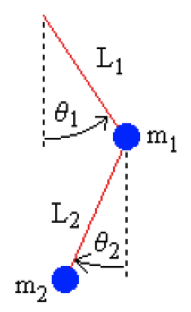
\includegraphics[scale=1]{energy.png}
		\caption{Energie im Pendel}
		\label{fig:energy}
	\end{minipage}
	\begin{minipage}[!t]{\textwidth}
		\vspace{0pt}\raggedright
		$x$ = Horizontale Position des Massenschwerpunkts\\
		$y$ = Vertikale Position des Massenschwerpunkts\\
		$\theta$ = Winkel\\
		$L$ = Pendellänge
	\end{minipage}
\end{figure}

Ausgangslage für die Berechnung ist das obere Pendel. Das erste Pendel wird als $1$ definiert mit $x1$ und $y1$. Äquivalent dazu wird das zweite Pendel als $2$ definiert mit $x2$ und $y2$.

Als erstes werden die einfachen trigonometrischen Gleichungen aufgestellt:

\begin{tabularx}{\textwidth}{X X}
	\begin{equation} \label{eq:energy:1_1}
		x_1 = L_1\sin\theta_1
	\end{equation}
	&
	\begin{equation} \label{eq:energy:1_2}
		y_1 = -L_1\cos\theta_1
	\end{equation}
\end{tabularx}

\begin{tabularx}{\textwidth}{X X}
	\begin{equation} \label{eq:energy:2_1}
		x_2 = x_1 + L_2\sin\theta_2
	\end{equation}
	&
	\begin{equation} \label{eq:energy:2_2}
		y_2 = y_1 - L_2\sin\theta_2
	\end{equation}
\end{tabularx}

\
und die erste (Geschwindigkeit) und zweite Ableitung (Beschleunigung) der Gleichung erstellt.

\begin{tabularx}{\textwidth}{X X}
	\begin{equation} \label{eq:energy:1_1}
		x'_1 = L_1\sin\theta_1
	\end{equation}
	&
	\begin{equation} \label{eq:energy:1_2}
		y'_1 = -L_1\cos\theta_1
	\end{equation}
\end{tabularx}

\begin{tabularx}{\textwidth}{X X}
	\begin{equation} \label{eq:energy:2_1}
		x_2 = x_1 + L_2\sin\theta_2
	\end{equation}
	&
	\begin{equation} \label{eq:energy:2_2}
		y_2 = y_1 - L_2\sin\theta_2
	\end{equation}
\end{tabularx}

\begin{tabularx}{\textwidth}{X X}
	\begin{equation} \label{eq:energy:1_1}
		x_1 = L_1\sin\theta_1
	\end{equation}
	&
	\begin{equation} \label{eq:energy:1_2}
		y_1 = -L_1\cos\theta_1
	\end{equation}
\end{tabularx}

\begin{tabularx}{\textwidth}{X X}
	\begin{equation} \label{eq:energy:2_1}
		x_2 = x_1 + L_2\sin\theta_2
	\end{equation}
	&
	\begin{equation} \label{eq:energy:2_2}
		y_2 = y_1 - L_2\sin\theta_2
	\end{equation}
\end{tabularx}

\subsubsection{Kräfte im Doppelpendel}
Die Kräfte werden pro Pendel berechnet und in einzelne Gleichungen gesetzt.
Folgende Variablen wurden definiert:

\begin{figure}[H]
	\begin{minipage}[!b]{0.4\textwidth}
		\centering
		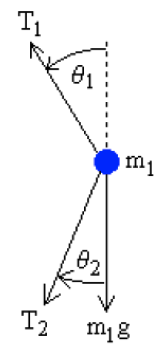
\includegraphics[scale=1]{force.png}
		\caption{Kräfte im Pendel}
		\label{fig:force}
	\end{minipage}
	\begin{minipage}[!t]{\textwidth}
		\vspace{0pt}\raggedright
		$T$ = Kraft im Pendel\\
		$m$ = Masse\\
		$g$ = Gravitations Konstante
	\end{minipage}
\end{figure}

Auf Grundlage des Newton Gesetzes wurden folgende Gleichungen für das obere Pendel erstellt:

\begin{equation} \label{eq:force:1_1}
	m_1 x_1'' = -T_1\sin\theta_1 + T_2\sin\theta_2
\end{equation}

\begin{equation} \label{eq:force:1_2}
	m_1 y_1'' = T_1\cos\theta_1 + T_1\cos\theta_2 - m_1 g
\end{equation}

und für das untere Pendel:
\begin{equation} \label{eq:force:2_1}
	m_2 x_2'' = -T_2\sin\theta_2
\end{equation}

\begin{equation} \label{eq:force:2_2}
	m_2 y_2'' = T_2\cos\theta_2 - m_2 g
\end{equation}

\subsubsection{Umformen der Gleichungen}
Um zu der entgültigen Differenziellen Gleichung für die Berechnung zu gelangen müssen die einzelnen Gleichungen algebraisch umgeformt werden.
Angefangen bei den Kräftegleichungen. Gleichung (\ref{eq:force:2_1}) und (\ref{eq:force:2_2}) werden nach $T_2\sin\theta_2$ bzw.nach $T_2\cos\theta_2$ aufgelöst und in die Gleichungen (\ref{eq:force:1_1}) und (\ref{eq:force:1_2}) eingesetzt.



(4.17) wird mit $\cos\theta_1$ und (4.18) mit $\sin\theta_1$ erweitert und nach $T_1\sin\theta_1\cos\theta_1$ aufgelöst.

Daraus ergibt sich die erste Teil der Bewegungsgleichung.


Um den zweiten Teil der Gleichung zu erhalten wird die Gleichung (4.15) mit $\cos\theta_2$ und die (4.16) mit $\sin\theta_2$ erweitert.


Der zweite Teil der Gleichung heisst somit


$x_2''$, $x_2''$, $y_1''$ und $y_2''$ werden durch die Gleichungen (4.9 – 4.12) ersetzt und mit Hilfe des Lagrange-Formalismus nach $\theta_1''$ und $\theta_2''$ aufgelöst. 


Die endgültige Bewegungsgleichung für das Doppelpendel lautet somit:
\begin{equation} \label{eq:final:1}
	\theta_1'' = \frac{-g(2m_1+m_2)\sin\theta_1 - m_2 g \sin(\theta_1 - 2\theta_2) -2\sin(\theta_1 - \theta_2)m_2({\theta_2'}^2 L_2 + {\theta_1'}^2 L_1\cos(\theta_1 - \theta_2))}
	{L_1(2m_1 + m_2 - m_2 \cos(2\theta_1 - 2\theta_2))}
\end{equation}

\begin{equation} \label{eq:final:1}
	\theta_2'' = \frac{2\sin(\theta_1 - \theta_2)({\theta_1'}^2 L_1(m_1 + m_2) + g(m_1 + m_2)\cos\theta_1 + {\theta_2'}^2 L_2 m_2 \cos(\theta_1 - \theta_2))}
	{L_2 (2m_1 + m_2 - m_2 \cos(2 \theta_1 - 2\theta_2))}
\end{equation}

\subsection{Numerische Differentialgleichung}
Die obige Bewegungsgleichung lässt sich aber noch nicht mittels des Runge-Kutta Algorithmus numerisch annähern. Um dies zu ermöglichen muss bedacht werden, dass die erste Ableitung von $\theta$ die Winkelgeschwindigkeit $\omega$ ist.

Somit ist:
$\theta_1' = \omega_1$
und
$\theta_2' = \omega_2$

und damit erhält man für den Runge-Kutta Algorithmus nun folgende Schlussgleichungen:
\begin{equation} \label{eq:rk:1}
	\theta_1' = \omega_1
\end{equation}
\begin{equation} \label{eq:rk:2}
	\theta_2' = \omega_2
\end{equation}

\begin{equation} \label{eq:rk:3}
	\omega_1' = \frac{-g(2m_1+m_2)\sin\theta_1 - m_2 g \sin(\theta_1 - 2\theta_2) -2\sin(\theta_1 - \theta_2)m_2(\omega_2^2 L_2 + \omega_1^2 L_1\cos(\theta_1 - \theta_2))}
	{L_1(2m_1 + m_2 - m_2 \cos(2\theta_1 - 2\theta_2))}
\end{equation}

\begin{equation} \label{eq:rk:4}
	\omega_2' = \frac{2\sin(\theta_1 - \theta_2)(\omega_1^2 L_1(m_1 + m_2) + g(m_1 + m_2)\cos\theta_1 + \omega_2^2 L_2 m_2 \cos(\theta_1 - \theta_2))}
	{L_2 (2m_1 + m_2 - m_2 \cos(2 \theta_1 - 2\theta_2))}
\end{equation}

\subsection{Numerisches Verfahren zur Berechnung der Lösung}
\subsubsection{Runge-Kutta Algorithmus} \label{cpt:rk}
Mittels des Runge-Kutta Verfahren kann eine Differenzialgleichung Numerisch approximiert werden. Das Verfahren eignet sich besonders gut für Berechnungen in einem Programm, da es sich um ein Iteratives Verfahren handelt und somit sehr einfach und Ressourcenschonend implementiert werden kann.
Verwendet wird das Runge-Kutta Verfahren 4. Ordnung auch RK4 genannt.

\newpage
\section{Umsetzung}
\subsection{Verwendete Technologien}
\subsubsection{OO-Sprache AS3}
Das Programm wird mittels Action Script 3 und dem Flex SDK in Eclipse Programmiert. Das Programm ist dank dem Flashplayer auf fast jedem Betriebssystem und Browser lauffähig.
Die Implementierung mittels Flex und AS3 ist speziell empfehlenswert, da das Framework schon viele Methoden für die Animation von Sprites beinhaltet und es dadurch zu massiven Zeit Einsparung kommt.

\subsubsection{Nummerisches Verfahren}
Um die Fehlerkommulierten Abweichungen der Berechnung auf möglichst lange Zeit klein zu halten wird das Numerische Verfahren von Runge-Kutta in der 4. Ordnung verwendet. Der Rechenaufwand für dieses Verfahren ist höher als bei anderen Verfahren wie z.B. dem Euler-Verfahren. Seine Genauigkeit auf grosse Zeitintervalle gleichen diesen Mehraufwand wieder aus. Auf den Algorithmus des Verfahren wird in Kapitel \ref{cpt:rk} genauer  eingegangen.

\newpage
\section{Software}
\subsection{Grafische Oberfläche}
Die Grafische Oberfläche wird als Skalierbares Modell aufgebaut. Der Vorteil in diesem Aufbau besteht darin, dass die Applikation auf jeder Bildschirmauflösung optimal dargestellt wird. Die Simulation des Pendels passt sich anhand der Fenstergrösse automatisch an.

\newpage
\listoffigures

\bibliographystyle{plainnat}
\bibliography{books}

\end{document}  